% chapter4.tex
% LED Chapter (Muon?)
As described in Chapter \ref{chap:muon}, the four extra modules added in 2010 covering the gap of veto system are equipped with LEDs. M7 and M8 have three LEDs: one at the center and the other two at two ends. M15 and M16 both have one LED installed at the center. The LEDs send out pulses every eight hours. The LED data are used to perform a stability controll of the $\upmu$-veto system. They are clearly defined comparing to muon induced events, therefore the LED events are good probe to estimate the long term stability of these four modules.
\section{Data selection}
The data of muon-veto Run70 to Run138 are used to analyze the aging effect of the veto system. This corresponds to a date from 24.08.2010 to 28.03.2017. When converting the raw data to ROOT-format, the events induced by LED firing are flagged. Therefore, they are easily separated from other events.
The LEDs fire three times every day. Each LED fires 60 pulses in one minute and they fire one after another, which also allows a separation of signals from different LEDs in M7 and M8.



\section{Long term stability}
The LEDs are fixed on the modules, so the energy spectrum is not smeared by the position dependent light readout. Also, the LEDs are supposed to have constant light output over short time. Thus the spectrum can be fitted with a gaussian function to get the average ADC values of several series.
To increase the statistical power of a single point, events of nine shot series (three days) are combined to perfom a gaussian fit. An example of such fit is illustrated in fig.\ref{fig:gaussian-fit}.

\begin{figure}[ht!]
  \centering
  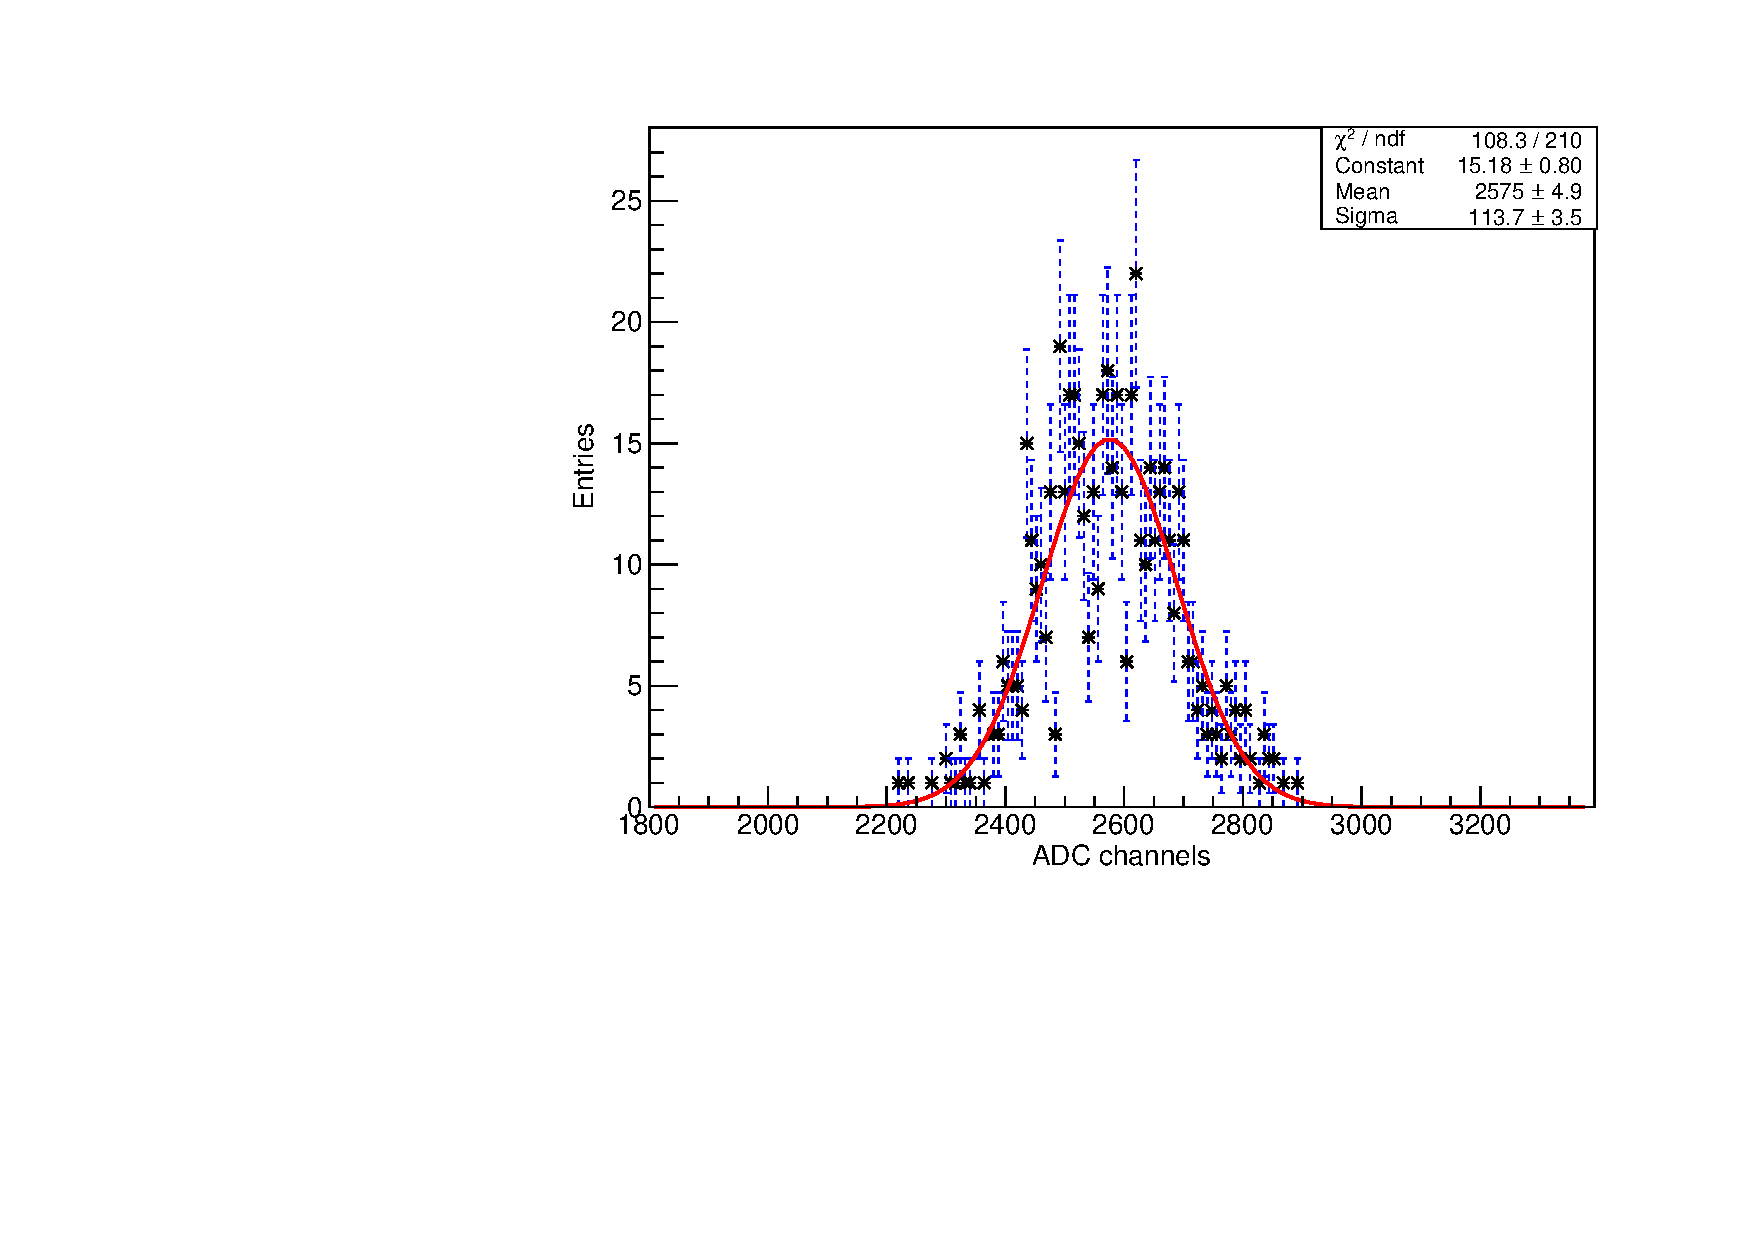
\includegraphics[width=0.6\textwidth{}]{./fig/gaussianM8.pdf}
  \caption{Example of an gaussian fit to nine LED fire series in Module 8, north PMT group. The spectrum is fitted with log likelihood method in ROOT.}
  \label{fig:gaussian-fit}
\end{figure}

The mean ADC values obtained from each gaussian fit are plotted over time. A change of these values over time could be due to various effects, e.g. decrease of the LED light output, aging of scintillator modules, problem of the PMTs or readout elctronics. To identify the contribution of different factors, the values are plotted separately for two PMT groups and three LEDs (for M7 and M8). Linear regressions are made for each data set, see fig.\ref{fig:M8LED}. The lines with different color represent the data from different LEDs.

As can be seen in the figure, the mean ADC values of two off-center LEDs differ about 1000 canals from the far end to the near end. Since M7 and M8 are ongly half the length of other top modules, such position dependent effect are even more significant in other modules.

In fig.\ref{fig:M8LED} , the error bar of a single data point is the statistical error given by the gaussian fit. Since most LED events in one fire serie have good gaussian form, the statistical error is mostly much smaller than the actually error. Several other effects lead to the fluctuation of the ADC value, for example,

\begin{table}
  \caption{}
  \label{}
  \begin{tabular}{c c c c c}

  \end{tabular}

\end{table}





\begin{figure}[ht]
  \centering
  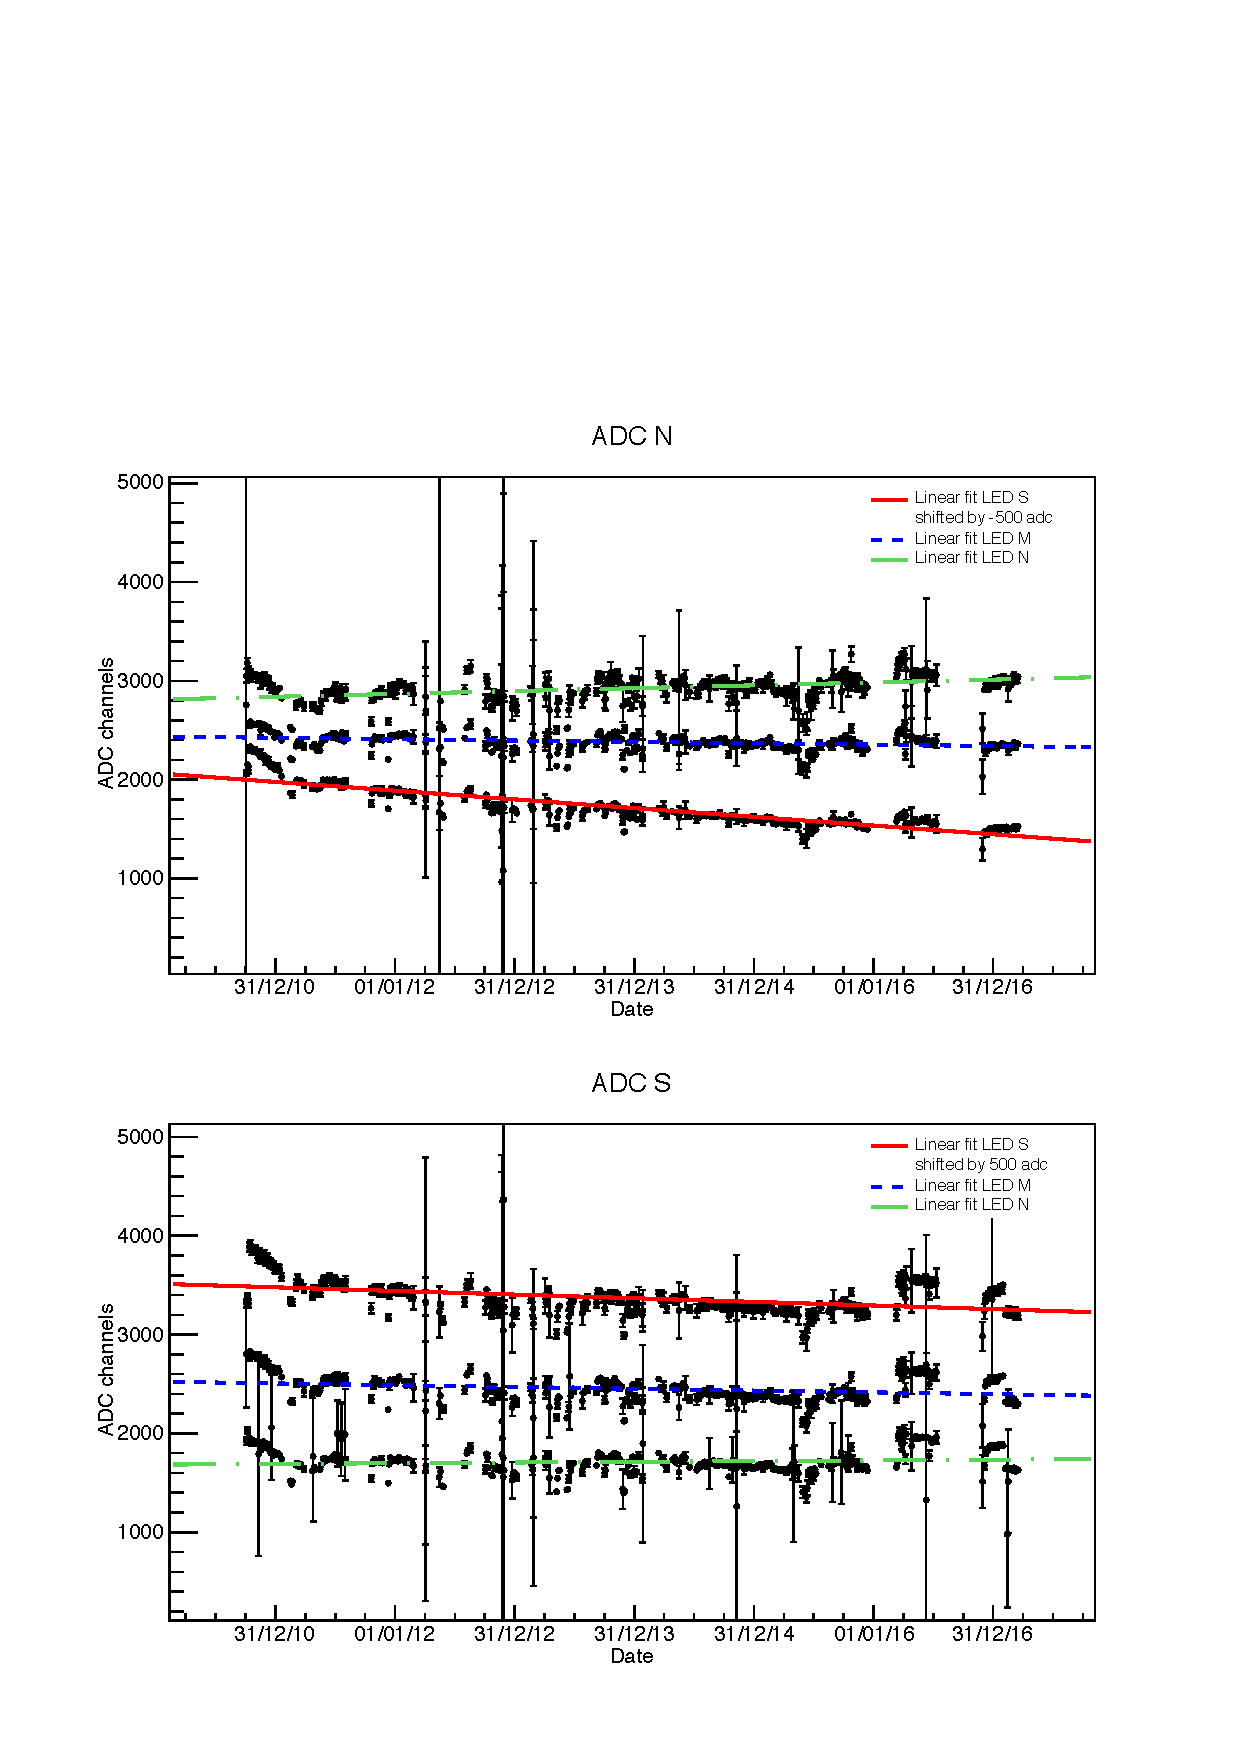
\includegraphics[width=0.9\textwidth{}]{./fig/M8LED.pdf}
  \caption{\textbf{The ADC values of LED signals over time in Module 8.}} The energy deposit of LED signals in ADC channels from Run70 to Run138 are plotted separately for 2 PMT groups (north in upper chart, south in lower chart). The trend of ADC values of different LEDs over time are approximated by linear fits: the green line (LED north), the blue line (LED middle), and the red line (LED south). For clarity reasons, the signals of the south LED are decreased by 500 channels in upper chart and increased by 500 in lower chart.
  \label{fig:M8LED}
\end{figure}
